\chapter{Udviklingsproces}
Arbejdes forløbet har været præget af nogle forskellige arbejdes former, disse former vil blive beskrevet i detaljer hvordan gruppen har benyttet sig af dem.

\section{Gennemførelse}
Projektet er gennemført i iterationer, i alt fire. Hver iteration indeholder en design- og implementeringsfase. Nedenfor her beskrives hver iteration. Alle gruppens medlemmer har arbejdet tæt sammen under hele forløbet.

\subsection{Iterativt udvikling}
Da projektet blev opdelt i use cases var det meget naturligt at opdele projektet i iterationer og derved starte med det mest grundlæggende funktionalitet først. Der blev planlagt fire iterationer. 

\textbf{Iteration 1}\\
Den første iteration i forløbet omhandlede systemet mest grundlæggende funktionalitet. Batteri, ESC'er, motorer og ultralyds sensorer tilsluttes dronen. Desuden gøres dronen i stand til at kunne oprette forbindelse til webapplikation via 3G-shield'et. Målet med iterationen var at opfylde use case 1. De efterfølgende iterationer bygger oven på denne iteration.

\textbf{Iteration 2}\\
Iteration 2's hovedformål var at få kommunikation mellem webapplikation og drone til at fungere. Bruger skulle også kunne oprette nye flyveopsætning  og sende dem til dronen. Ydermere skulle drone kunne finde egen GPS position, flyvehøjde og orientering. Ud fra viden om egen position, flyvehøjde og orientering skulle dronen kunne flyve til de forudbestemt lokationer af brugeren. Til denne iteration var use case 2 og 3 tildelt.

\textbf{Iteration 3}\\
Iteration 3's hovedformål var det primære fokus billeder. Der skulle monteres kamera på dronen, så den kunne tage billeder ved de lokationer som bruger havde defineret. Alle billeder taget under flyvning sendes via mobilnet fra dronen til serveren og gøres tilgængelige for bruger. Målet med iteration 3 var at udføre use case 4 og 5.

\textbf{Iteration 4}\\
Iteration 4's hovedformål var at udvikle anti kollision til dronen. Inden tilføjelsen af anti kollision kunne dronen udelukkende flyve i lukkede områder uden forhindringer. Tilføjelsen af anti kollision ville muliggøre flyvning i normale områder med forhindringer. Målet med iteration 4 var at udføre use case 6.

\section{Metoder}

\subsection{RUP model}
\textbf{R}ational \textbf{U}nified \textbf{P}rocess er blevet anvendt til at holde den overordnet fremgangs metode til projektet.  

\begin{figure}[H]
	\centering
	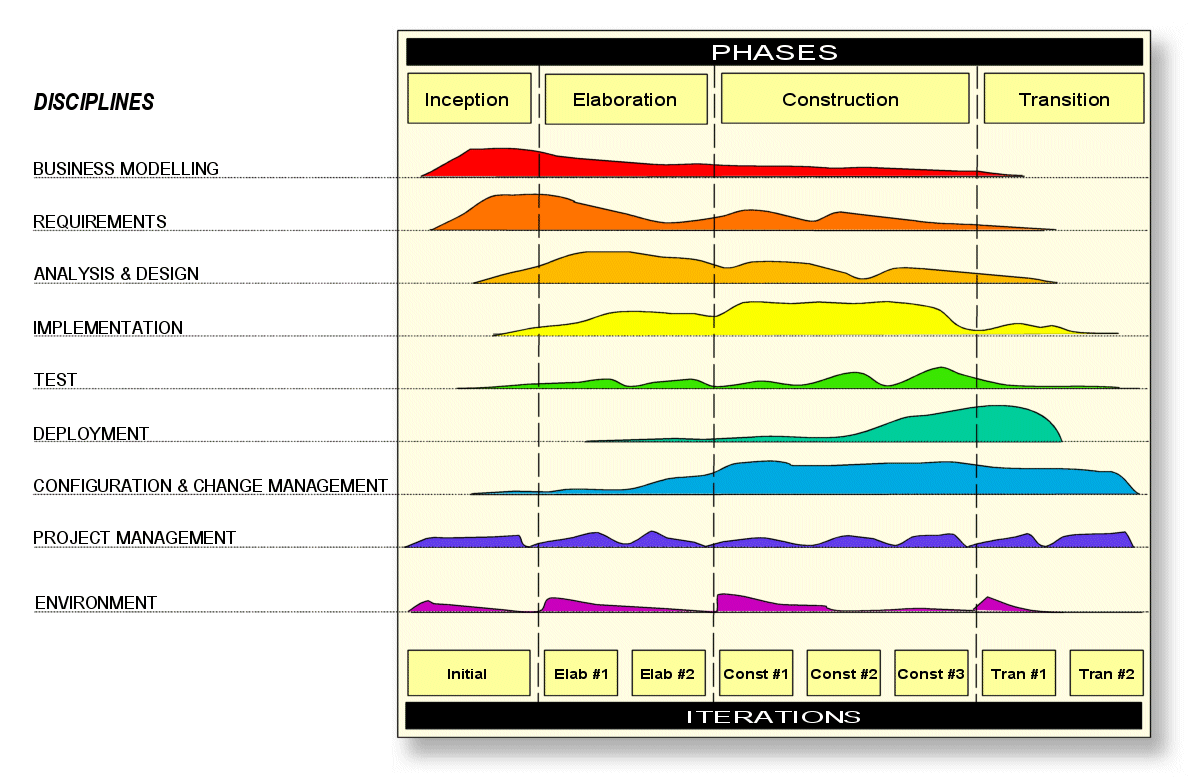
\includegraphics[width=0.60\textwidth]{Billeder/Udviklingsproces/RUP}
	\caption{RUP model}
	\label{fig:rup}
\end{figure}

\textbf{Inception}\\
I denne fase blev de indledende dokumenter udarbejdet. Der blev lavet forundersøgelse og valg vedrørende hardware. En indkøbs liste blev også udarbejdet i denne fase. Krav til systemet blev også udarbejdet i denne fase samt en overordnet systemskitse. 

\textbf{Elaboration}\\
I denne fase blev domain modellen udarbejdet, der blev fortaget en use case analyse af systemets funktionalitet. Ved brug af use case analysen blev der også udarbejdet en iterations plan over den kommende udvikling af systemet. 

\textbf{Construction}\\
I denne fase var produktet i fokus. Udviklingen forgik skiftevis mellem implementering af nyt funktionalitet, test og dokumentation af færdiggjort funktionalitet.

\textbf{Transition}\\
I denne fase blev der gjort opsamling af dokumentationen og rapporten samt accepttest.

\subsection{N + 1 model}
Dokumentationen af dette projekt har fulgt dokumentations modelle N + 1. N + 1 modellen er en dokumentations model for software, modelle deler dokumentationen af software systemet op i forskellige view's. Til dette projekt er det blevet benyttet 5 + 1 modelle. 5 + 1 modellen indeholder use case view, logical view, process view, data view, deployment view og implementation view. De nævnte view's vil blive beskrevet mere i dybden nedenfor. 

\begin{figure}[H]
	\centering
	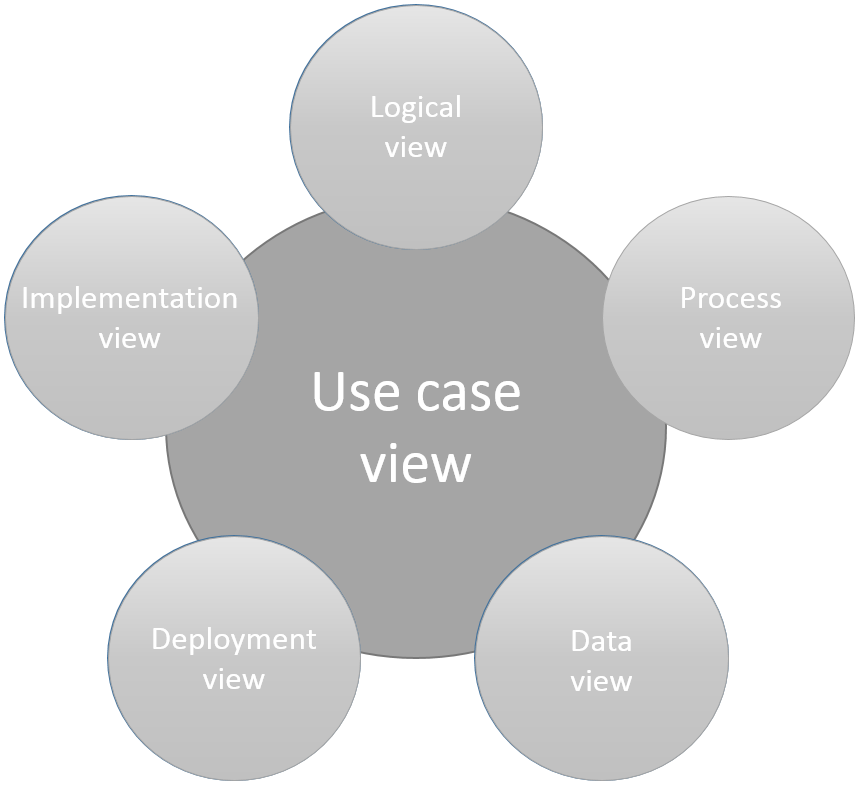
\includegraphics[width=0.60\textwidth]{Billeder/Udviklingsproces/n+1}
	\caption{n + 1 modellen}
	\label{fig:n+1}
\end{figure}

\textbf{Use Case View}\\
Dette view er benyttet på baggrund af opdelings muligheder af projektet. View'et giver også et mere håndgribeligt overblik over systemet, da fokus i view'et ligger på funktionalitet for brugeren af systemet. Under dette view i dokumentationen finde use case diagrammer, hvilket tydeliggøre sammenhæng imellem aktør, bruger og systemet.

\textbf{Logical View}\\
Dette view er benyttet til at beskrive de logiske blokke i systemet.

På baggrund af hver iteration i systemet er der udarbejdet dertilhørende pakke-, klasse- og sekvensdiagrammer. Dette giver et overblik over systemets funktionalitet på programmerings niveau.

\textbf{Deployment View}\\
Dette view er benyttet til at beskrive det fysiske elementer i systemet. Her beskrives også hvor de forskellige pakker befinder sig i systemet. Hvilket protokoller som er anvendt som interface imellem de forskellige enheder er også beskrevet i dette view.

\textbf{Process View}\\
Dette view er benyttet til at beskrive hvilke sideløbende processer der befinder sig i systemet. I view'et findes også beskrivelse af kommunikations timing, da i nogle tilfælde i forbindelse med kommunikation er det vigtigt at kommunikationen bliver afviklet i en bestemt rækkefølge.

\textbf{Data View}\\
Dette view er benyttet til at beskrive databasen i systemet. Håndteringen af dataen og hvordan den tilgås er også beskrevet i dette afsnit. 

\textbf{Implementation View}\\
Dette view er benyttet til at beskrive de vigtigste elementer i systemet som ikke er blevet beskrevet i de andre views. I dette view er opsættelse af systemet til vider udvikling og hvordan systemet kompileres beskrevet.

\subsection{Dokument udarbejdelse}
I kombination med RUP arbejdsmetoden og ASE modellen som ses på figur \ref{fig:dokument_udvikling} er dokumentationen opdelt i fire dokumenter, hvilket giver et godt overblik over de forskellige dokumenter tilhørende projektet. Software delen af dokumentationen er så yderligere opdelt efter modellen n + 1 som beskrevet .

\begin{figure}[H]
	\centering
	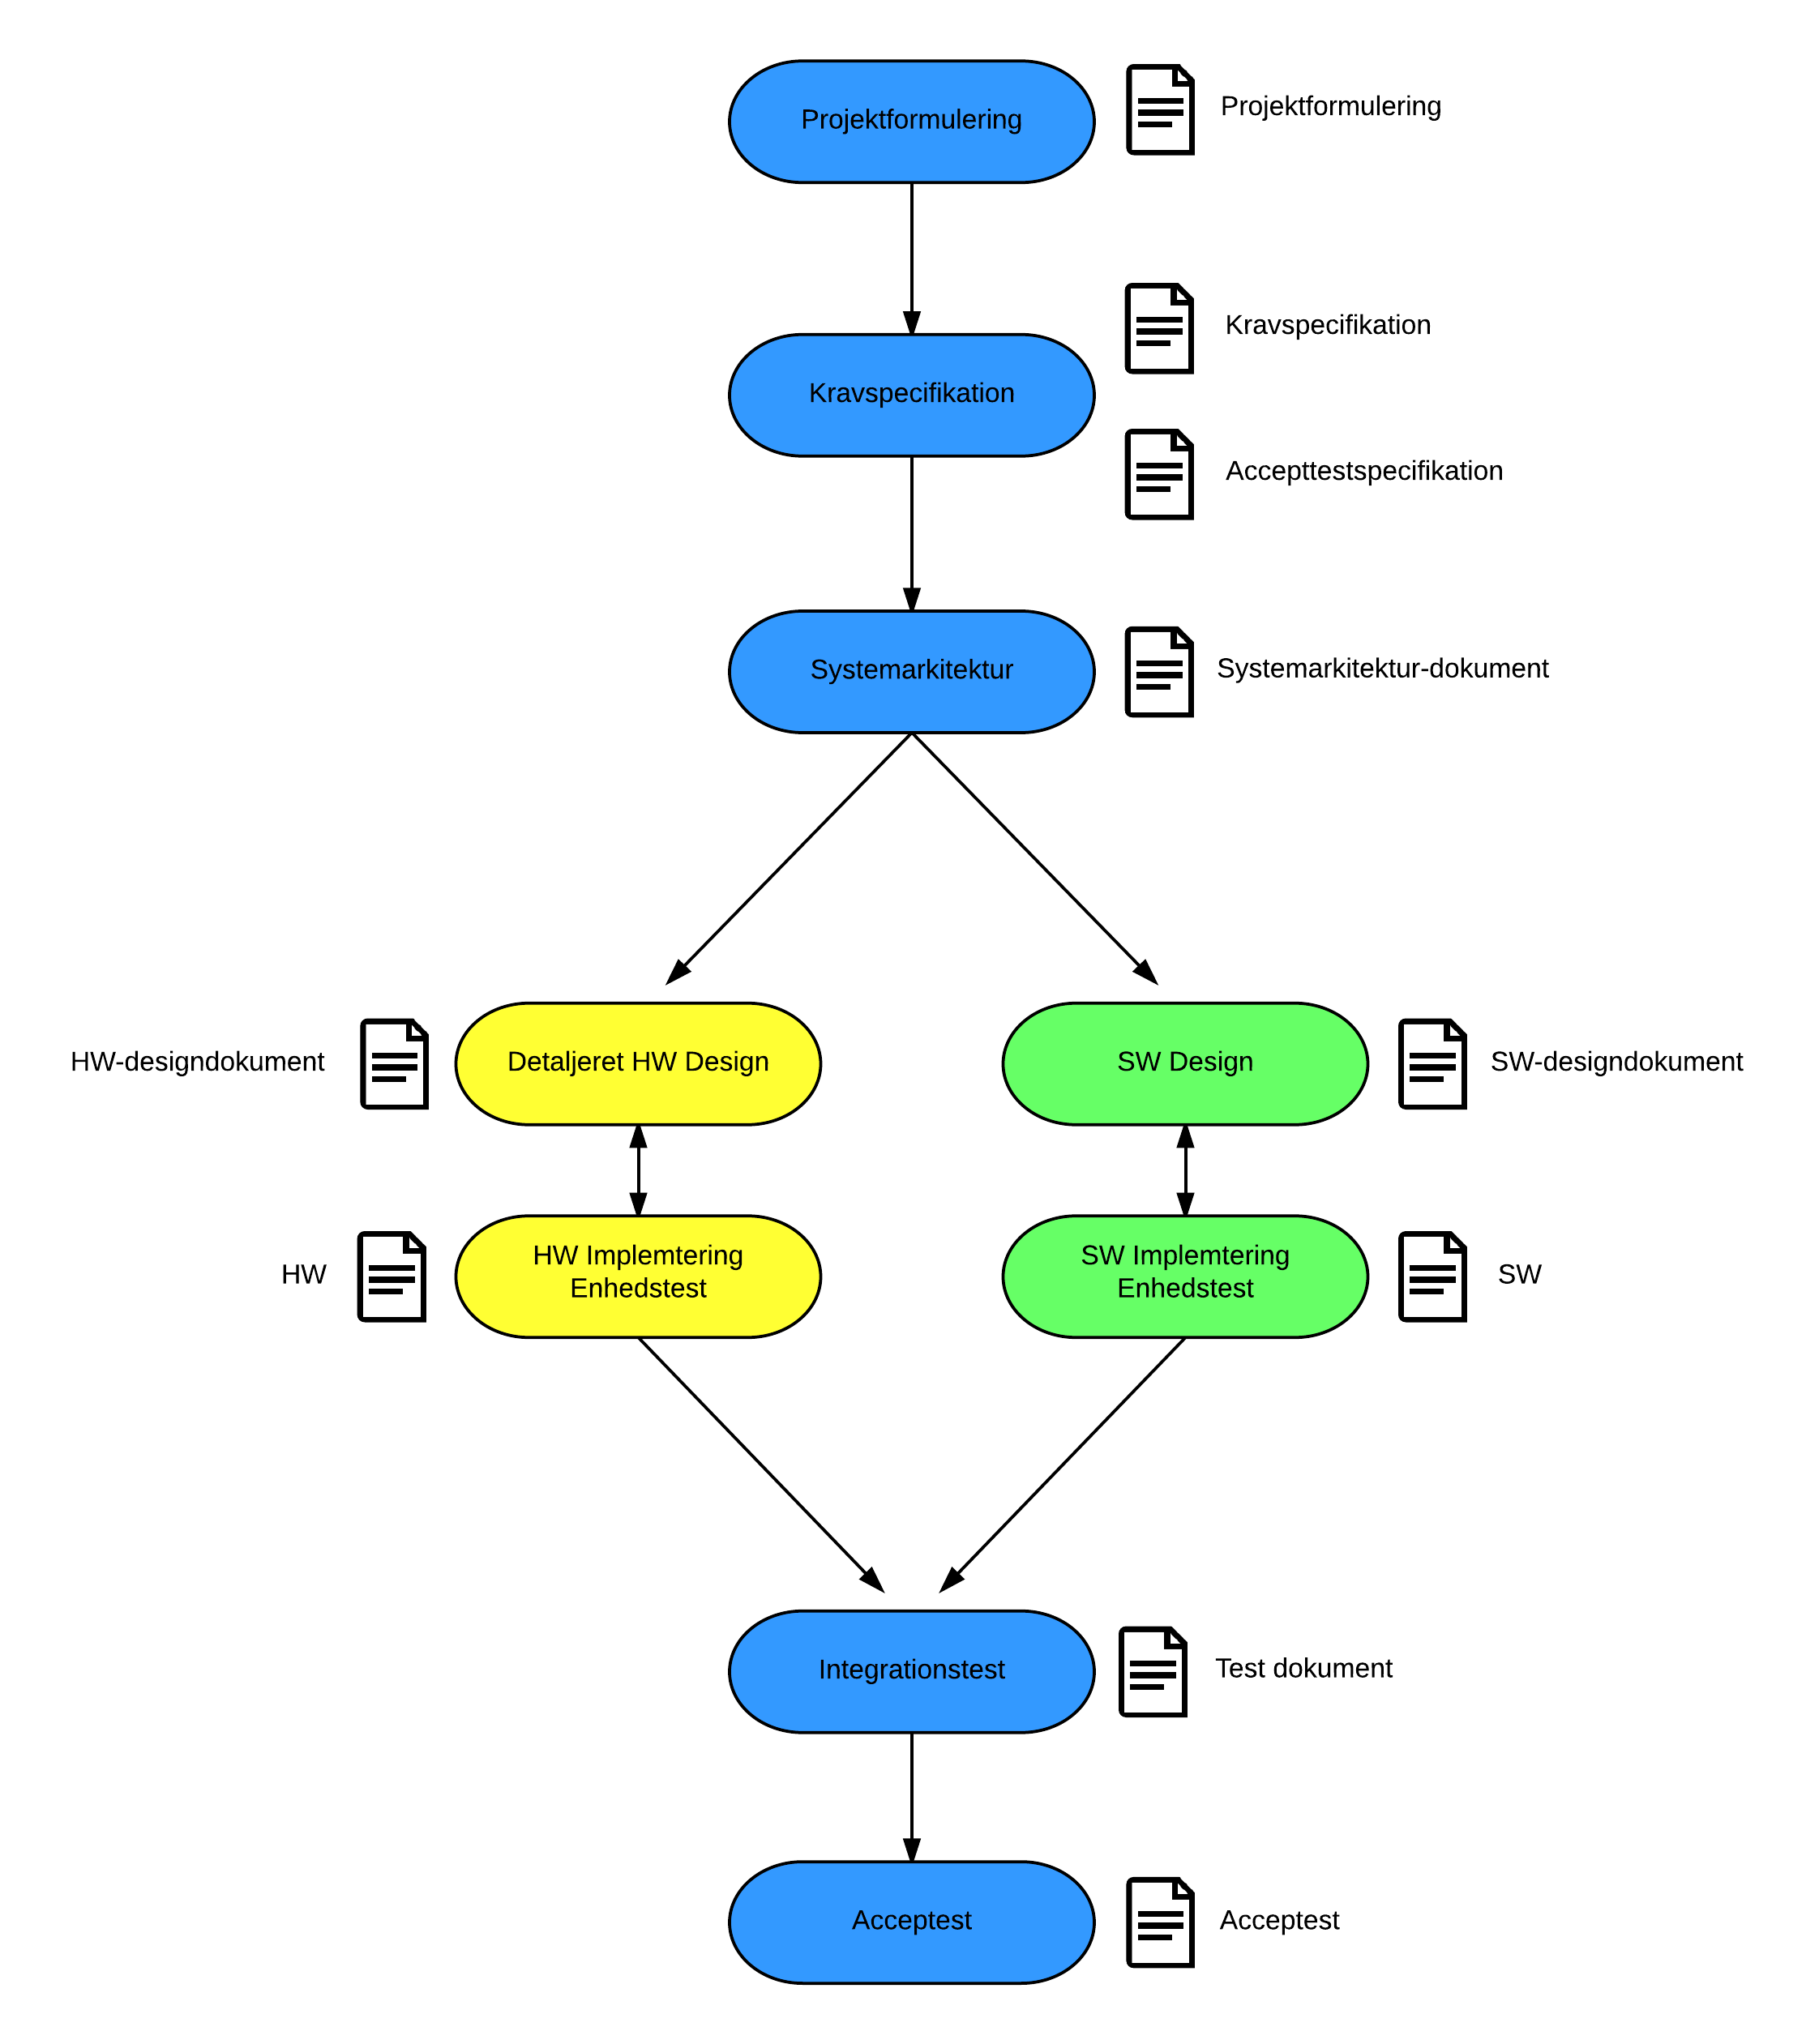
\includegraphics[width=1\textwidth]{Billeder/Udviklingsproces/ase_model}
	\caption{ASE modellen}
	\label{fig:dokument_udvikling}
\end{figure}

\subsection{Agile arbejdsmetoder}
Udviklingen og dokumentationen af produktet har også været meget præget af agile arbejdsmetoder. Metoder som scrum er blevet delvis anvendt i forløbet. Under construction fasen blev scrum meetings brugt og en samlet backlog blev benyttet til at bevare overblik over projektets fremgang.

\section{Diagrammer}
Til dokumentationen af projektet er der benyttet en række diagrammer, disse diagrammer vil blive beskrevet i dette afsnit.

\textbf{Use case}\\
Use cases og dertilhørende diagrammer er benyttet i forløbets indledende faser, til at overskueliggøre projektets omfang og opdele projektet i mindre dele. Use casene har fungeret som omdrejnings punkt i projektet, det er her funktionaliteten udspringer fra.

\textbf{Domainmodel}\\
I de indledende faser blev der også udarbejdet en domainmodel som blev brugt til at finde ansvars områder i projektet.

\textbf{SysML}\\
SysMLl diagrammerne er blevet benyttet til dokumentation af hardwaren til projektet. Disse diagrammer er blevet anvendt til at tydeliggøre, hvilke hardware blokke der høre til hvor og hvordan de kommunikere sammen.  

\textbf{UML}\\
UML diagrammerne er blevet  benyttet til dokumentation af softwaren. Disse diagrammer er blevet anvendt til at forklare hvordan systemet er opbygget, hvordan de forskellige delsystemer snakker sammen og hvordan funktionaliteten er opbygget.